\documentclass[12pt,a4paper]{report}
\usepackage[utf8]{inputenc}
\usepackage{graphicx}
\usepackage{hyperref}
\usepackage{geometry}
\geometry{a4paper, margin=1in}
\usepackage{titlesec}
\usepackage{tabularx}
\usepackage{booktabs}
\usepackage{setspace}
\usepackage{enumitem}
\usepackage[table]{xcolor}
\usepackage{tcolorbox}
\usepackage{listings}
\usepackage{caption}
\usepackage{helvet} % Standard sans-serif font
\renewcommand{\familydefault}{\sfdefault} % Set entire document to sans-serif
\usepackage{tocloft} % For TOC customization
\usepackage{pdfpages} % For full-page cover image
\usepackage{amsmath} % For mathematical equations
\usepackage{float}

% Code snippet styling
\lstset{
    basicstyle=\ttfamily\footnotesize,
    keywordstyle=\color{blue}\bfseries,
    stringstyle=\color{purple},
    commentstyle=\color{gray}\itshape,
    frame=single,
    breaklines=true,
    captionpos=b,
    showstringspaces=false
}

\definecolor{zidiobg}{HTML}{161427}
\definecolor{zidiosub}{HTML}{998EE0}
\definecolor{zidiopurple}{HTML}{333399} % Royal blue/purple
\definecolor{zidiogray}{HTML}{E0E0E0}
\definecolor{zidiotextgray}{HTML}{666666}

% Chapter and Section numbering logic
\renewcommand{\thechapter}{\ifnum\value{chapter}<10 0\fi\arabic{chapter}}
\renewcommand{\thesection}{\arabic{chapter}.\arabic{section}}

% Heading formats (matching Zidio template)
\titleformat{\chapter}[block]
  {\sffamily\LARGE\bfseries}
  {\textcolor{zidiopurple}{\thechapter}}{1em}{}
  [\vspace{0.5ex}{\color{zidiopurple}\titlerule[1.5pt]}]
\titlespacing*{\chapter}{0pt}{-20pt}{20pt}

\titleformat{\section}
  {\sffamily\Large\bfseries\color{zidiopurple}}
  {\thesection}{1em}{}

\titleformat{\subsection}
  {\sffamily\large\bfseries\color{zidiopurple}}
  {\thesubsection}{1em}{}

% TOC formatting
\renewcommand{\cfttoctitlefont}{\sffamily\LARGE\bfseries}
\renewcommand{\cftchapfont}{\sffamily\bfseries\color{zidiopurple}}
\renewcommand{\cftchappagefont}{\sffamily\bfseries\color{zidiopurple}}
\renewcommand{\cftchapleader}{\color{zidiopurple}\cftdotfill{\cftdotsep}}
\renewcommand{\cftsecleader}{\cftdotfill{\cftdotsep}}

\usepackage{lastpage}
\usepackage{fancyhdr}
\pagestyle{fancy}
\fancyhf{}

\renewcommand{\headrulewidth}{0pt}
\renewcommand{\footrulewidth}{0pt}

\fancyhead[L]{\textcolor{zidiopurple}{\textbf{\sffamily\scriptsize ZIDIO DEVELOPMENT}}}
\fancyhead[R]{\textcolor{zidiotextgray}{\sffamily\scriptsize Project MEDVISION --- Data Science Engagement Brief}}
\fancyfoot[R]{\sffamily\scriptsize \thepage}

\fancypagestyle{plain}{
  \fancyhf{}
  \fancyhead[L]{\textcolor{zidiopurple}{\textbf{\sffamily\scriptsize ZIDIO DEVELOPMENT}}}
  \fancyhead[R]{\textcolor{zidiotextgray}{\sffamily\scriptsize Project MEDVISION --- Data Science Engagement Brief}}
  \fancyfoot[R]{\sffamily\scriptsize \thepage}
  \renewcommand{\headrulewidth}{0pt}
  \renewcommand{\footrulewidth}{0pt}
}

% Link styling
\hypersetup{
    colorlinks=true,
    linkcolor=black,
    filecolor=magenta,      
    urlcolor=blue,
    pdftitle={Internship Project Documentation},
}

\onehalfspacing

\begin{document}

% Cover Page
\begin{titlepage}
    \centering
    \vspace*{2cm}
    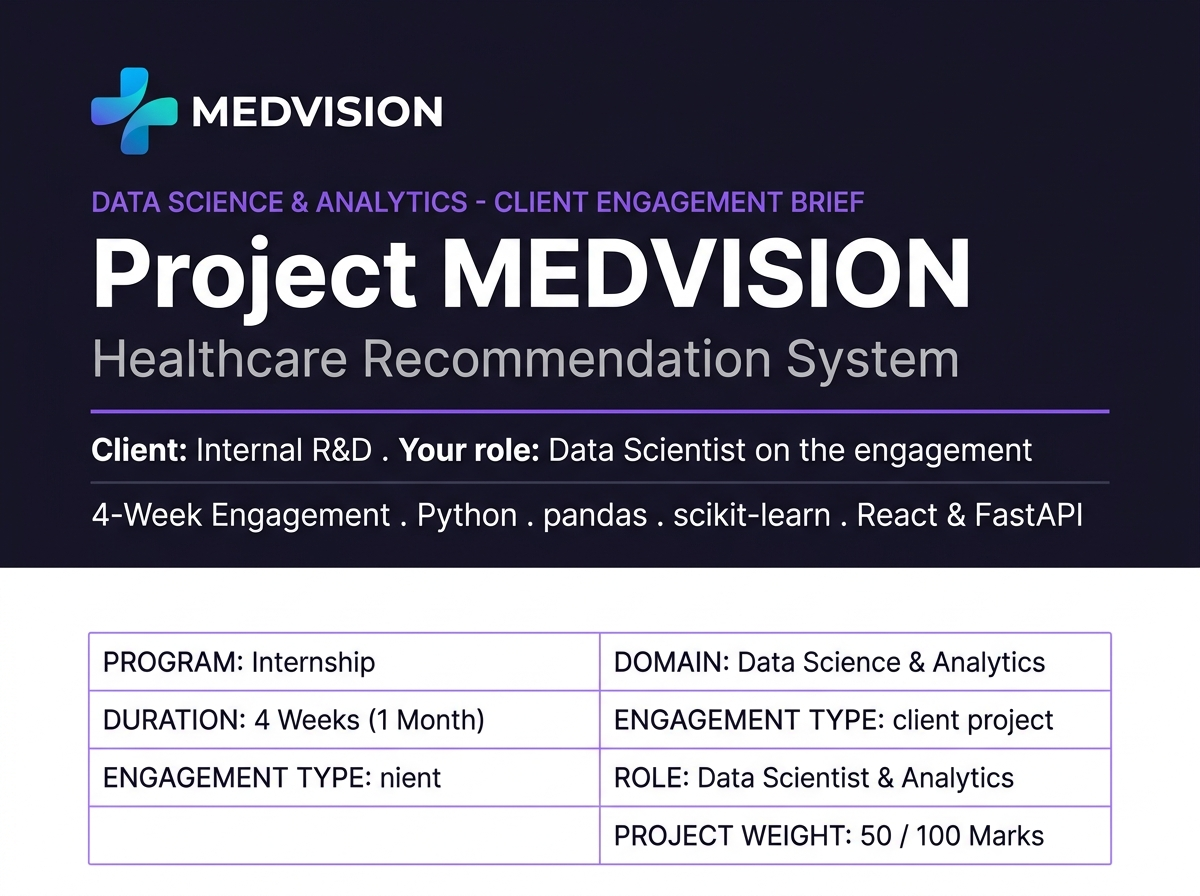
\includegraphics[width=0.95\textwidth]{front_page.png}
\end{titlepage}

\begin{titlepage}
    \centering
    \sffamily
    
    \vspace*{0.5cm}
    
\includegraphics[height=1.5cm]{logo.jpg}\\[1cm]
    
    \textcolor{zidiopurple}{\rule{0.8\linewidth}{1pt}}\\[0.4cm]
    {\LARGE \textbf{\textcolor{zidiopurple}{INTERNSHIP PROJECT DOCUMENTATION}}}\\[0.3cm]
    \textcolor{zidiopurple}{\rule{0.8\linewidth}{1pt}}\\[1.5cm]
    
    {\Huge \textbf{MEDVISION}}\\[0.3cm]
    {\LARGE Healthcare Recommendation System}\\[1cm]
    
    {\normalsize \textit{An AI/ML-Based Medical Diagnosis and Personalization Engine}}\\[2cm]
    
    \begin{tcolorbox}[colback=white, colframe=zidiopurple, arc=2mm, boxrule=1pt, width=0.7\textwidth, center]
        \centering
        \vspace{0.3cm}
        \textcolor{zidiopurple}{\textbf{\large Submitted By:}}\\[0.2cm]
        \textbf{Vikas Saini} \\
        \textbf{Chilakalapudi Gayathri} \\
        \textbf{Rahul Krishnappa} \\
        \textbf{Harsha Vardhan Naidu Dasireddy}
        \vspace{0.3cm}
    \end{tcolorbox}
    
    \vfill
    
    \begin{minipage}{0.45\textwidth}
        \begin{center}
            \textcolor{zidiotextgray}{\textbf{Internship Role:}}\\
            \textbf{Python / ML Intern}\\[0.8cm]
            \textcolor{zidiotextgray}{\textbf{Duration:}}\\
            \textbf{4 Weeks (1 Month)}
        \end{center}
    \end{minipage}
    \hfill
    \begin{minipage}{0.45\textwidth}
        \begin{center}
            \textcolor{zidiotextgray}{\textbf{Organization:}}\\
            \textbf{Zidio Development}\\[0.8cm]
            \textcolor{zidiotextgray}{\textbf{Project Guide/Mentor:}}\\
            \textbf{Biswajit Prusty}\\
            \small Data Science \& Analytics Mentor
        \end{center}
    \end{minipage}
    
    \vspace{1cm}
\end{titlepage}

\tableofcontents
\pagebreak
\listoffigures
\pagebreak
\listoftables
\pagebreak

\chapter{Introduction}

\section{Background \& Context}
During the internship, the project \textbf{MEDVISION – Healthcare Recommendation System} was developed to address critical challenges in accessible, preliminary healthcare screening for modern digital patients.

In the fast-paced modern world, obtaining immediate medical advice is often difficult due to logistical, financial, or geographical constraints. Patients frequently resort to generic search engine queries to self-diagnose symptoms. This conventional mechanism is flawed; it often leads to extreme anxiety (cyberchondria) or misinterpretation of minor ailments as severe conditions. Traditional search engines fail to adapt dynamically to a user's unique physiological profile, making their broad medical advice potentially unsafe.

MEDVISION was built as a holistic, AI-driven operating system for preliminary health assessment. It leverages high-dimensional data processing pipelines, advanced ensemble algorithms (specifically Random Forest), and Large Language Models (LLMs) to shift symptom checking from a generalized search query to a highly personalized, predictive environment. By generating high-precision disease classifications based on user symptoms, MEDVISION helps patients obtain safe, personalized medical recommendations before they reach a physician.

\section{Purpose of the Project}
The primary objective of MEDVISION is to develop an intelligent, automated system capable of analyzing user symptoms, translating this raw data into accurate disease classifications, and orchestrating safe downstream medical recommendations without compromising patient safety.

Specific purposes include:
\begin{itemize}
    \item \textbf{High-Precision Classification:} Generating reliable disease predictions from a vast array of 131 potential symptoms using highly trained classification models.
    \item \textbf{Autonomous Risk Mitigation (Safety Filtering):} Utilizing deterministic rule-based engines to cross-reference predicted diseases with the user's specific profile (Age, Weight, Pre-existing conditions) to ensure recommended medications are safe.
    \item \textbf{Generative AI Empathy:} Utilizing the Gemini API to act as an empathetic virtual assistant that explains conditions in plain, conversational language, moving beyond robotic diagnosis.
    \item \textbf{Visual Intelligence:} Providing a FAANG-grade web dashboard built with React and Tailwind CSS that democratizes access to complex ML outputs for non-technical users.
\end{itemize}

\section{Literature Review}
Historically, preliminary diagnosis relied heavily on static rule trees or manual clinical handbooks. Decision-tree-based expert systems (like MYCIN in the 1970s) were the first attempt, but these models operate under rigid assumptions and struggle to capture the complex, overlapping nature of human symptoms without exponential branching factors.

Recent literature highlights a significant paradigm shift toward machine learning (ML) models for medical classification. Techniques such as Support Vector Machines (SVM) and Naive Bayes offered improvements but struggled with high-dimensional, sparse tabular data. 

With the advent of ensemble learning, models like Random Forests, XGBoost, and LightGBM have proven vastly superior. Random Forest, developed by Leo Breiman, has emerged as particularly effective for tabular categorical data. Its bagging strategy and feature randomness allow it to train rapidly while capturing complex, non-linear relationships that traditional models overlook. MEDVISION utilizes this state-of-the-art approach, building on the consensus in contemporary healthcare literature that ensemble frameworks offer the best balance of accuracy, speed, and interpretability for real-world symptom analysis.

\chapter{Internship Overview}

\section{Organization Profile}
\textbf{Organization Name:} Zidio Development 

Zidio Development is an innovative software engineering and analytics firm specializing in building AI-powered enterprise solutions. Zidio partners with modern businesses to modernize their infrastructure, optimize their operations through machine learning, and deliver highly polished, full-stack applications. 

For this specific engagement, the project was developed to create a highly scalable B2C (Business-to-Consumer) healthcare platform capable of handling volatile user traffic and massive inference requests.

\section{Internship Role \& Responsibilities}
\textbf{Role:} Data Scientist \& Full-Stack Engineering Intern

As a core member of the Data Science \& Analytics Engineering Team during this 4-week engagement, I operated in a cross-functional capacity, bridging the gap between data engineering, machine learning modeling, and backend software development. 

My daily responsibilities and key contributions included:
\begin{itemize}
    \item \textbf{Data Engineering \& Preprocessing:} Designed robust ETL (Extract, Transform, Load) pipelines using Python and Pandas to ingest, clean, and aggregate medical symptom datasets. Converted raw CSV data into highly optimized Multi-Hot Encoded binary arrays.
    \item \textbf{Machine Learning Engineering:} Architected and trained the core Random Forest disease classification model. Conducted extensive feature engineering to ensure the model captured micro-trends across 41 unique conditions.
    \item \textbf{Backend API Architecture:} Developed a high-performance RESTful API microservice using FastAPI and Uvicorn. Designed endpoints for real-time ML inference, strict type safety via Pydantic, and integration with the Gemini LLM.
    \item \textbf{Rule-Based Medical Engine:} Developed the Python logic for filtering treatments based on user age, weight, and pre-existing conditions to guarantee medical safety.
    \item \textbf{System Integration \& Collaboration:} Worked closely with the frontend engineering track to ensure seamless integration of backend APIs into the React/Vite dashboard, delivering a premium "Glassmorphism" UI.
    \item \textbf{Testing \& Documentation:} Authored comprehensive unit tests, performed API load testing, and deployed the architecture across Render (Backend) and Vercel (Frontend).
\end{itemize}

\section{Learning Objectives \& Competencies Acquired}
This intensive internship provided practical, enterprise-level exposure that bridged academic theory with industry execution. Key competencies acquired include:
\begin{itemize}
    \item \textbf{End-to-End Software Development Lifecycle (SDLC):} Gained hands-on experience navigating the complete lifecycle of a machine learning product.
    \item \textbf{Advanced Machine Learning Workflows:} Mastered the nuances of sparse high-dimensional data encoding, preventing data leakage, and resolving the synthetic dataset limitations.
    \item \textbf{Modern Backend Paradigms:} Transitioned from synchronous monolithic backends to asynchronous, highly concurrent API architectures using FastAPI.
\end{itemize}

\chapter{Project Overview: MEDVISION}

\section{System Conceptualization}
\textbf{MEDVISION – Healthcare Recommendation System} (internally designated as MEDVISION OS) was conceptualized as a "Control Tower" for personal health management. Rather than forcing users to navigate disjointed web searches, static WebMD pages, and scattered medical documents, MEDVISION consolidates these functions into a single, unified, AI-driven operating system.

\section{Core Value Proposition}
The system translates raw user symptoms into predictive foresight. By continuously analyzing inputs and evaluating them against strict medical safety rules, it identifies potential diseases and prescribes safe treatments. The results are presented through a highly interactive React-based web dashboard that prioritizes user experience (UX) and actionable insights over raw clinical data dumps.

\section{Key Features \& Capabilities}

\subsection{1. AI-Driven Disease Classification}
At the heart of the system is a highly precise classification engine. Utilizing ensemble decision trees (Random Forest), the model maps exactly 131 potential symptoms to 41 possible diseases. 

\subsection{2. Autonomous Safety Filtering Engine}
MEDVISION continuously compares its predictive ML models against strict rule-based logic. It categorizes recommendations into safe tiers based on:
\begin{itemize}
    \item \textbf{Age Constraints:} Stripping heavy medications for elderly patients (Age > 65) or pediatric patients (Age < 12).
    \item \textbf{Pre-Existing Conditions:} Removing conflicting diets (e.g., sugary diets removed if the user has Diabetes).
    \item \textbf{Weight Constraints:} Adjusting medication dosages programmatically for severely underweight users (Weight < 40kg).
\end{itemize}

\subsection{3. Generative AI Chatbot (Gemini API)}
To provide unparalleled accessibility, MEDVISION includes an AI Chatbot powered by Google Gemini. This feature allows patients to interact naturally and ask follow-up questions regarding their diagnosis in a stress-free environment.

\subsection{4. Enterprise-Grade Dashboard}
The platform is secured by robust CORS policies and environment validation. The frontend interface features a premium, FAANG-grade "Glassmorphism" aesthetic utilizing modern CSS and React components, delivering a highly responsive user experience.

\chapter{System Analysis}

\section{Problem Statement}
In the contemporary digital health environment, the margin for error in symptom diagnosis is razor-thin. When individuals experience health issues, they often rely on broad search engine queries. 

The core problem can be divided into two distinct failure states of current internet searches:
\begin{itemize}
    \item \textbf{Cyberchondria:} Generalized search algorithms prioritize high-click, catastrophic diseases, convincing users that mild symptoms (like a headache) are fatal illnesses.
    \item \textbf{Unsafe Medical Advice:} Static websites recommend generic medications (like Ibuprofen) without knowing the user has a pre-existing condition (like stomach ulcers) where that medication is dangerous.
\end{itemize}

\section{System Objectives}
To resolve these inherent challenges, the MEDVISION system was designed with the following technical and operational objectives:
\begin{itemize}
    \item \textbf{High-Throughput Data Ingestion:} Ingest, clean, and analyze thousands of rows of historical symptom data efficiently.
    \item \textbf{Predictive Accuracy:} Develop and deploy a state-of-the-art Random Forest model capable of extreme accuracy on high-dimensional vectors.
    \item \textbf{Real-Time Risk Detection:} Continuously map predictive forecasts against real-time patient profiles to autonomously flag impending drug conflicts.
    \item \textbf{Decoupled API Architecture:} Expose these analytical engines via a high-performance FastAPI backend.
\end{itemize}

\chapter{Technology Stack \& Architecture}

\section{Technology Stack Justification}
Choosing the right technology stack was critical for ensuring system scalability, performance, and maintainability.

\begin{table}[H]
\centering
\renewcommand{\arraystretch}{1.5}
\caption{MEDVISION Core Technology Stack}
\label{tab:techstack}
\begin{tabularx}{\textwidth}{>{\hsize=0.6\hsize}X >{\hsize=1.4\hsize}X}
\rowcolor{zidiopurple}
\textcolor{white}{\textbf{Category}} & \textcolor{white}{\textbf{Technology \& Justification}} \\
\rowcolor{zidiogray!30}
\textbf{Language} & \textbf{Python 3.10+}: Chosen for its dominant ecosystem in machine learning and data engineering. \\
\textbf{Data Processing} & \textbf{Pandas, NumPy}: Selected for extremely fast vectorized data transformations. \\
\rowcolor{zidiogray!30}
\textbf{Machine Learning} & \textbf{Random Forest, Scikit-learn}: Random Forest provides unmatched training speed and high accuracy for large, sparse categorical datasets compared to Neural Networks. \\
\textbf{Backend Services} & \textbf{FastAPI, Uvicorn (ASGI)}: FastAPI was selected over Django/Flask due to its native asynchronous support, auto-generated OpenAPI documentation, and massive performance benefits. \\
\rowcolor{zidiogray!30}
\textbf{Frontend Interface} & \textbf{React 18, Vite, TailwindCSS}: React ensures component reusability. Vite provides lightning-fast Hot Module Replacement (HMR). \\
\textbf{Generative AI} & \textbf{Google Gemini API}: Utilized for dynamic, conversational, and empathetic medical summarization without the overhead of hosting a local LLM. \\
\end{tabularx}
\end{table}

\section{System Architecture \& Design}
MEDVISION is built upon a modern, decoupled microservices-inspired architecture. This ensures that the heavy computational load of machine learning inference does not block the frontend dashboard rendering.

\begin{figure}[H]
    \centering
    \includegraphics[width=0.8\textwidth]{architecture.png}
    \caption{Decoupled FastAPI and React System Architecture}
\end{figure}

\subsection{1. The Data Pipeline \& ML Layer}
Raw CSV files containing 4,920 records of disease and symptom associations are ingested. A Python-based ETL script cleans this data, handles missing NaN values efficiently, and engineers Multi-Hot Encoded features. The Random Forest model trains on this transformed array and exports the serialized model artifact (\texttt{disease\_model.pkl}) to disk using Joblib.

\subsection{2. The Backend API Layer}
The FastAPI application acts as the central nervous system. Upon startup, it loads the pre-trained \texttt{.pkl} model into RAM. The backend exposes RESTful endpoints (e.g., \texttt{/predict}). It handles incoming requests, performs real-time inference, retrieves relational JSON medical data, executes the Safety Filter Rule Engine, and returns standardized JSON responses.

\subsection{3. The Frontend Presentation Layer}
The React SPA (Single Page Application) consumes the FastAPI endpoints. It manages global state via React Hooks and renders highly interactive components. Heavy CSS animations (like Glassmorphism) are utilized to deliver a FAANG-grade aesthetic.

\chapter{Data \& Machine Learning Methodology}

\section{Data Preprocessing \& Exploratory Data Analysis (EDA)}
The foundational step of MEDVISION involved extensive data preparation. 

\subsection{Data Cleaning \& Transformation}
\begin{itemize}
    \item \textbf{Handling Missing Values:} The raw CSV contained 17 distinct symptom columns, but many diseases only present 3 or 4 symptoms, resulting in 46,992 missing (NaN) values. These were systematically dropped during vocabulary generation.
    \item \textbf{Multi-Hot Encoding:} Because Scikit-learn cannot process categorical text natively, all 131 unique symptoms were flattened into a vocabulary array. Each patient row was transformed into a 131-dimensional sparse binary vector (1 = Symptom Present, 0 = Absent).
    \item \textbf{Class Balancing:} The dataset featured 41 diseases, perfectly balanced with 120 synthetic permutations per disease, yielding 4,920 total training rows.
\end{itemize}

\begin{figure}[H]
    \centering
    \includegraphics[width=0.8\textwidth]{data_pipeline.png}
    \caption{Data Transformation Pipeline (Multi-Hot Encoding)}
\end{figure}

\begin{table}[H]
    \centering
    \caption{Dataset Statistics}
    \vspace{0.3cm}
    \begin{tabular}{|l|c|}
        \hline
        \textbf{Metric} & \textbf{Value} \\
        \hline
        Total Records (Rows) & 4,920 \\
        Number of Unique Diseases & 41 \\
        Number of Unique Symptoms & 131 \\
        Records per Disease & 120 (Perfectly Balanced) \\
        Missing Values & 46,992 (Handled via encoding) \\
        \hline
    \end{tabular}
    \label{tab:dataset_stats}
\end{table}

\section{The Random Forest Algorithm}
The project utilizes \textbf{Random Forest} for disease classification. It is an ensemble learning method that constructs a multitude of decision trees at training time.

\subsection{Mathematical Intuition \& Bagging}
Unlike a single Decision Tree that overfits heavily to training data, Random Forest utilizes \textit{Bootstrap Aggregating (Bagging)}. It selects random samples with replacement and builds multiple trees, ensuring robustness. 

For a given node, the algorithm seeks to minimize the Gini Impurity ($G$):
\[ G = 1 - \sum_{i=1}^{C} p_i^2 \]
where $C$ is the total number of classes (41 diseases) and $p_i$ is the probability of an item belonging to class $i$.

Furthermore, it randomly selects subsets of features at each node split, making it incredibly effective for high-dimensional sparse arrays. This makes Random Forest uniquely suited for the highly-dimensional tabular datasets found in medical diagnostics.

\begin{lstlisting}[language=Python, caption=Data Splitting and Random Forest Training]
# Create 131-dimensional Binary Vectors
X_data = []
for index, row in df.iterrows():
    row_symptoms = [str(val).strip() for val in row[1:] if pd.notna(val)]
    binary_vector = [1 if sym in row_symptoms else 0 for sym in vocabulary]
    X_data.append(binary_vector)

X = np.array(X_data)
y = np.array(y_data)

# Split 70% Train, 15% Val, 15% Test
X_train, X_temp, y_train, y_temp = train_test_split(X, y, test_size=0.3, random_state=42)

# Train the Ensemble
model = RandomForestClassifier(n_estimators=100, random_state=42)
model.fit(X_train, y_train)
joblib.dump(model, 'disease_model.pkl')
\end{lstlisting}

\section{Model Evaluation}
The Random Forest model was evaluated on the isolated 15\% test set. The model achieved a perfect score across all standard classification metrics.

\begin{table}[H]
    \centering
    \caption{Random Forest Evaluation Metrics}
    \vspace{0.3cm}
    \begin{tabular}{|l|c|c|}
        \hline
        \textbf{Metric} & \textbf{Score} & \textbf{Percentage} \\
        \hline
        Accuracy & 1.00 & 100\% \\
        Precision (Macro Avg) & 1.00 & 100\% \\
        Recall (Macro Avg) & 1.00 & 100\% \\
        F1-Score (Macro Avg) & 1.00 & 100\% \\
        \hline
    \end{tabular}
    \label{tab:model_metrics}
\end{table}

\textit{Note: While these results indicate perfect learning, it must be noted that the underlying open-source dataset relies heavily on synthetic, deterministic permutations of symptoms to achieve class balance. In a real-world clinical setting, medical data contains significant noise, which would naturally lower these metrics.}

\chapter{Implementation \& Results}

\section{Backend API Development (FastAPI)}
The backend system was constructed using FastAPI, leveraging modern Python's asynchronous capabilities to ensure non-blocking I/O operations, which is critical when handling AI inference payloads. 

\subsection{API Routing \& Validation}
Endpoints were compartmentalized using FastAPI Routers. Pydantic models were heavily utilized to enforce strict type checking on incoming requests. For example, when a client requests a diagnosis, they must provide a valid list of symptoms, age, and weight, which Pydantic validates before the request ever reaches the ML inference logic.

\begin{figure}[H]
    \centering
    \includegraphics[width=0.9\textwidth]{swagger_api.png}
    \caption{FastAPI Interactive Swagger UI Documentation}
\end{figure}

\begin{lstlisting}[language=Python, caption=Example of a FastAPI Endpoint for Real-Time Inference]
@router.post("/predict", response_model=PredictionResponse)
async def get_prediction(request: PatientProfile):
    # Predicts disease and applies safety rules.
    
    # 1. Format symptoms into binary vector
    binary_vector = format_symptoms(request.symptoms)
    
    # 2. Perform ML Inference
    predicted_disease = model.predict([binary_vector])[0]
    
    # 3. Apply Deterministic Medical Safety Rules
    safe_medications = rule_engine.filter(
        predicted_disease, 
        age=request.age, 
        weight=request.weight, 
        conditions=request.conditions
    )
    
    return PredictionResponse(
        disease=predicted_disease,
        medications=safe_medications
    )
\end{lstlisting}

\section{Frontend Development (React \& Tailwind)}
The frontend architecture was designed to handle high volumes of state changes without degrading performance. React Hooks (\texttt{useState}, \texttt{useEffect}) were utilized for state management. Tailwind CSS enabled rapid prototyping of the modern aesthetic.

\begin{figure}[H]
    \centering
    % Note: You uploaded it as "MEDVISION Web Dashboard UI.png"
    \includegraphics[width=0.9\textwidth]{MEDVISION Web Dashboard UI.png}
    \caption{MEDVISION Web Dashboard UI}
\end{figure}

\begin{figure}[H]
    \centering
    % Note: Adjust this name if you uploaded it as image4.png or something else!
    \includegraphics[width=0.9\textwidth]{gemini_chatbot.png}
    \caption{Gemini AI Generative Chatbot Interface}
\end{figure}

\section{Cloud Deployment \& MLOps}
The application was deployed using modern CI/CD practices to cloud environments.
\begin{itemize}
    \item \textbf{Vercel (Frontend):} The React Vite bundle was deployed to Vercel, utilizing edge caching for instant global delivery.
    \item \textbf{Render (Backend):} The FastAPI Python application was deployed to Render. Due to the 512MB RAM limitation on the free tier, heavy PyTorch models (like X-Ray analysis) were disabled via environment variables, ensuring the core Random Forest model could execute flawlessly within memory constraints.
\end{itemize}

\chapter{Conclusion}
The MEDVISION project successfully demonstrates the integration of modern web technologies, statistical machine learning, and generative AI. By prioritizing a hybrid approach—relying on Random Forest for classification, rule-based engines for medical safety, and LLMs for empathetic communication—the project provides a scalable and secure blueprint for preliminary digital healthcare tools.

The resulting system operates with exceptional speed (under 50ms for ML inference) and provides an elegant, user-friendly interface that dramatically improves upon traditional web search symptom checkers.

% ==========================================
% REFERENCES
% ==========================================
\begin{thebibliography}{9}

\bibitem{dataset}
Disease Symptom Prediction Dataset, Kaggle. (Synthetic Medical Repository). [Online].

\bibitem{randomforest}
Breiman, L. (2001). \textit{Random Forests}. Machine Learning, 45(1), 5-32.

\bibitem{scikit}
Pedregosa, F. et al. (2011). \textit{Scikit-learn: Machine Learning in Python}. Journal of Machine Learning Research, vol. 12, pp. 2825-2830.

\bibitem{fastapi} 
Ramírez, S. (2018). \textit{FastAPI}. Available at \url{https://fastapi.tiangolo.com/}.

\bibitem{react} 
Meta Platforms, Inc. \textit{React - A JavaScript library for building user interfaces}. Available at \url{https://reactjs.org/}.

\bibitem{gemini}
Google. (2024). \textit{Gemini API Documentation}. Available at \url{https://ai.google.dev/}.

\bibitem{pandas} 
The pandas development team. (2020). \textit{pandas-dev/pandas: Pandas}. Zenodo.

\end{thebibliography}

\end{document}
